\documentclass[tikz,border=4pt]{standalone}
\usetikzlibrary{positioning}

\begin{document}
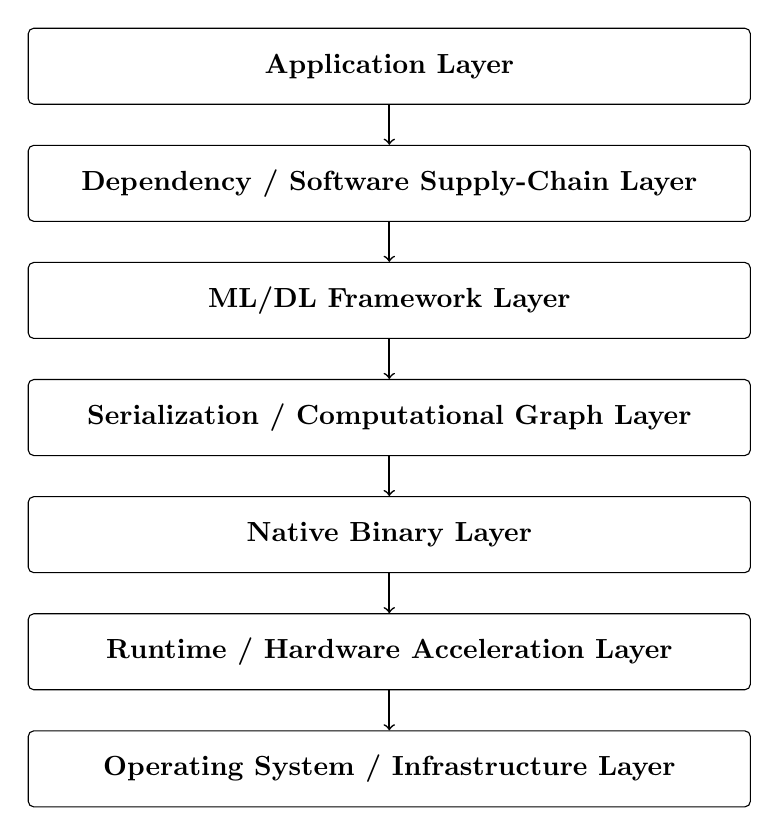
\begin{tikzpicture}[
  stage/.style={
    draw,
    rounded corners=2pt,
    text width=3.5in,
    minimum height=0.38in,
    align=center,
    font=\bfseries,
    inner sep=4pt
  },
  node distance=0.20in
]
\node[stage] (application) {Application Layer};
\node[stage, below=of application] (dependency) {Dependency / Software Supply-Chain Layer};
\node[stage, below=of dependency] (framework) {ML/DL Framework Layer};
\node[stage, below=of framework] (serialization) {Serialization / Computational Graph Layer};
\node[stage, below=of serialization] (binary) {Native Binary Layer};
\node[stage, below=of binary] (runtime) {Runtime / Hardware Acceleration Layer};
\node[stage, below=of runtime] (infrastructure) {Operating System / Infrastructure Layer};

\draw[->, semithick] (application) -- (dependency);
\draw[->, semithick] (dependency) -- (framework);
\draw[->, semithick] (framework) -- (serialization);
\draw[->, semithick] (serialization) -- (binary);
\draw[->, semithick] (binary) -- (runtime);
\draw[->, semithick] (runtime) -- (infrastructure);
\end{tikzpicture}
\end{document}
